\chapter*{Deep learning neural networks}\addcontentsline{toc}{chapter}{Deep learning neural networks}
\section{Context}
Deep learning neural networks gained popularity again in recent years, after the AI winter ended. Since then neural networks became part of the everyday life, we hear about artificial intelligence being used in smart phones to enhance images quality or recognize certain settings and take a picture accordingly. AI is also being used in cancer research and other fields of bioinformatics, and personal assistants became extremely popular.

But even with the seemingly endless capabilities of artificial neural networks we are far from creating anything that could pass the Turing test, let alone have the cognitive capacities of humans. This problem is AI-complete or AI-hard, meaning that creating a network that could keep up a human-like conversation would require data scientist and researchers to construct a universal artificial intelligence. A small but important step to achieve this is to create a system capable of doing simple reading comprehension tasks that also require some common sense knowledge.

The most common structures of these experimental neural networks include recurrent neural network layers and attention layers. Before we explain the function of these building-blocks we need to lay down a foundation.

\section{Basics}
Artificial neural networks are said to mimic the human neural networks, which is true on the surface, but mathematically speaking they are more like a complex mathematical functions that tries to predict an output with the given set of inputs.
\subsection{Perceptron}
Perceptrons are the binary linear classifying units of the neural network. They function like neurons (Figure~\ref{fig:neuron}) so to speak.
\begin{figure*}[!htb]
	\centering
	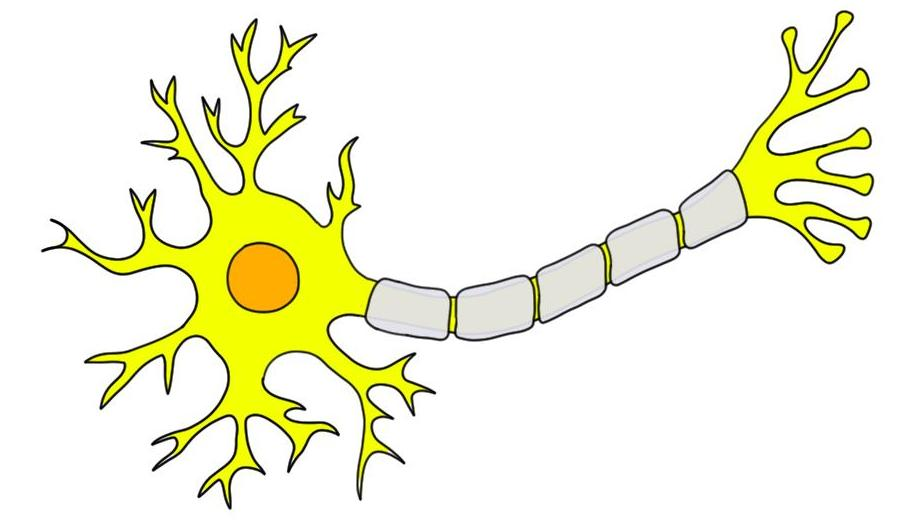
\includegraphics[scale=0.1]{neuron.jpg}
	\caption{Neurons are usually depicted like this. Image from the \textit{Neuroscientifically Challenged} website.}
	\label{fig:neuron}
\end{figure*}
Neurons fire if certain dendrites receive signals. Similarly, a perceptron "fires" if its input vector's weighted sum is above a certain bias.
\[output = \sum (input * weight) + bias\]
But what are these parameters?

The weight could be loosely explained like the strength of a given input, how much should it affect the output value. Bias is a threshold we set for the perceptron.
\subsection{Feed forward}
The layers of the neural network consist of these perceptrons. A simple structure is depicted in Figure~\ref{fig:neural_net}.
\begin{figure*}[!htb]
	\centering
	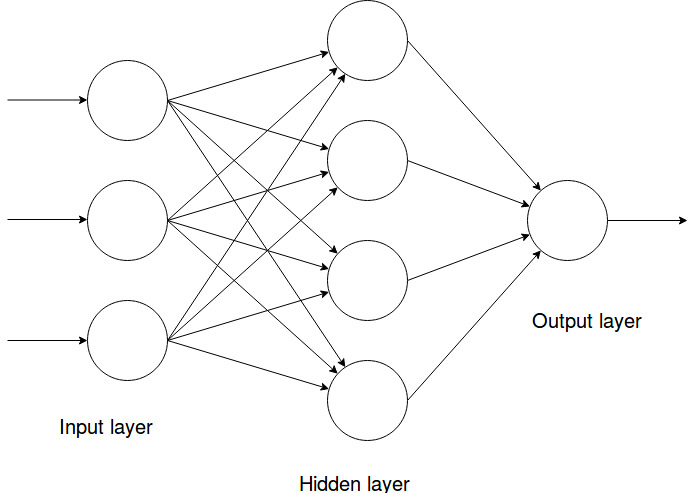
\includegraphics[scale=0.5]{simple_neural_network.jpg}
	\caption{A simple feed forward neural network.}
	\label{fig:neural_net}
\end{figure*}
This neural network consists of feed-forward layers, which means that every perceptron in each layer connects to every perceptron in the previous and the next layer. Each connection has a weight value attached to it. The output of this network is constructed as follows:
\[output = \sum activationFunction(\sum(input * weight_1 + bias_1)) * weight_2 + bias_2\]
Here the activation function is a function that the hidden layer's output passes through. It is used to add non-linearity to the network. This will be crucial in the backpropagation step.
There are multiple types of activation functions in deep learning, the most commons being tanh (Figure~\ref{fig:tanh}), sigmoid (Figure~\ref{fig:sigmoid}), relu and its variations.
\[tanh(x) = \frac{e^x - e^{-x}}{e^x + e^{-x}}\]
\begin{figure*}[!htb]
	\centering
	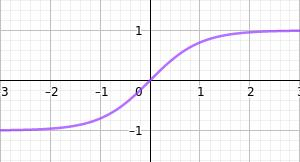
\includegraphics[scale=0.5]{tanh.jpg}
	\caption{Hyperbolic tangent activation function}
	\label{fig:tanh}
\end{figure*}
\[sigmoid(x) = \sigma(x) = \frac{1}{1 + e^{-x}}\]
\begin{figure*}[!htb]
	\centering
	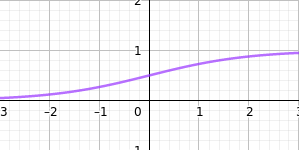
\includegraphics[scale=0.5]{sigmoid.jpg}
	\caption{Sigmoid activation function}
	\label{fig:sigmoid}
\end{figure*}
\[relu(x) = \begin{cases}x & \quad \text{if } x \geq 0 \\ 0 & \quad \text{else}\end{cases}\]
\begin{figure*}[!htb]
	\centering
	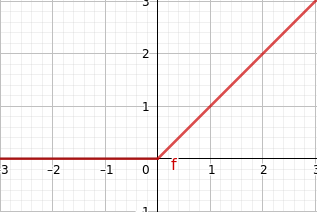
\includegraphics[scale=0.5]{relu.jpg}
	\caption{Rectified linear unit activation function}
	\label{fig:relu}
\end{figure*}
\subsection{Backpropagation}

\section{Natural Language Processing with Deep learning}
As mentioned above the kind of layers used in Natural Language Processing are mostly recurrent neural network layers and attention layers.
\subsection{Recurrent Neural Networks}
\subsubsection{Long-Short Term Memory}
\subsubsection{Gated recurrent unit}
\subsection{Attention}
The Attention mechanism was first described in (Bahdanau, 2015) and was used for machine translation. Since then it became a widely used tool in natural language processing. The idea behind this mechanism is that when the neural network predicts the output, it only uses parts of the given input instead of the full input. That is where the most relevant informations are concentrated and this mechanism only pays \textit{attention} to these parts.